% Standalone source for the hcinfer repository-level architecture diagram.
% Ported verbatim from hcinfer-stat/hcinfer-stat_v1b.tex (preamble lines
% 39 to 162 and the tikzpicture at lines 389 to 434). Compile with
% latexmk -pdf then convert to PNG with pdftools::pdf_convert at 300 DPI.
\documentclass[border=5pt]{standalone}
\usepackage{tikz}
\usetikzlibrary{arrows.meta,backgrounds,calc,fit,positioning,shapes.geometric}

\definecolor{codebg}{HTML}{F7F8FA}
\definecolor{codeframe}{HTML}{E1E5EA}
\definecolor{codetext}{HTML}{243746}
\definecolor{codemuted}{HTML}{7A8896}
\definecolor{codestring}{HTML}{2C5F8A}
\definecolor{hcink}{HTML}{243746}
\definecolor{hcpage}{HTML}{FFFFFF}
\definecolor{hcapi}{HTML}{2C5F8A}
\definecolor{hcapifill}{HTML}{F2F6FA}
\definecolor{hccorecol}{HTML}{3D6B5D}
\definecolor{hccorefill}{HTML}{F3F7F5}
\definecolor{hcobject}{HTML}{6A5D84}
\definecolor{hcobjectfill}{HTML}{F6F4F8}
\definecolor{hcsupport}{HTML}{8A8F94}
\definecolor{hcsupportfill}{HTML}{F7F8FA}
\definecolor{hcline}{HTML}{6D7680}
\definecolor{hcfaint}{HTML}{A9B2BA}

\tikzset{
  hcblock/.style={
    draw=hcink,
    rounded corners=3pt,
    line width=0.55pt,
    fill=hcpage,
    align=center,
    minimum height=7mm,
    inner xsep=6pt,
    inner ysep=3pt,
    font=\normalsize\bfseries\ttfamily,
    text=hcink
  },
  hcentry/.style={
    hcblock,
    fill=hcink,
    text=hcpage,
    minimum width=23mm
  },
  hccore/.style={
    hcblock,
    draw=hcapi,
    fill=hcapifill,
    text=hcapi,
    line width=0.75pt,
    minimum width=30mm
  },
  hcleaf/.style={
    hcblock,
    draw=hcapi,
    text=hcapi,
    minimum width=25mm,
    font=\scriptsize\bfseries\ttfamily
  },
  hcpanel/.style={
    draw=hcsupport,
    fill=hcsupportfill,
    rounded corners=8pt,
    line width=0.6pt,
    inner sep=7pt
  },
  hccard/.style={
    draw=hcsupport,
    fill=hcsupportfill,
    rounded corners=8pt,
    line width=0.6pt,
    text=hcink,
    align=left,
    text width=56mm,
    inner xsep=8pt,
    inner ysep=7pt,
    font=\small\sffamily
  },
  hcedge/.style={
    -{Stealth[length=2.2mm,width=1.6mm]},
    line width=0.55pt,
    color=hcline,
    rounded corners=6pt
  },
  hcinternaledge/.style={
    -{Stealth[length=1.9mm,width=1.3mm]},
    line width=0.42pt,
    color=hcfaint,
    densely dashed,
    rounded corners=5pt
  },
  hcsplit/.style={
    line width=0.35pt,
    color=hcfaint
  },
  hclabel/.style={
    font=\scriptsize\sffamily,
    text=hcline,
    align=center
  },
  hcgroup/.style={
    font=\scriptsize\sffamily\bfseries,
    text=hcink
  }
}

\begin{document}
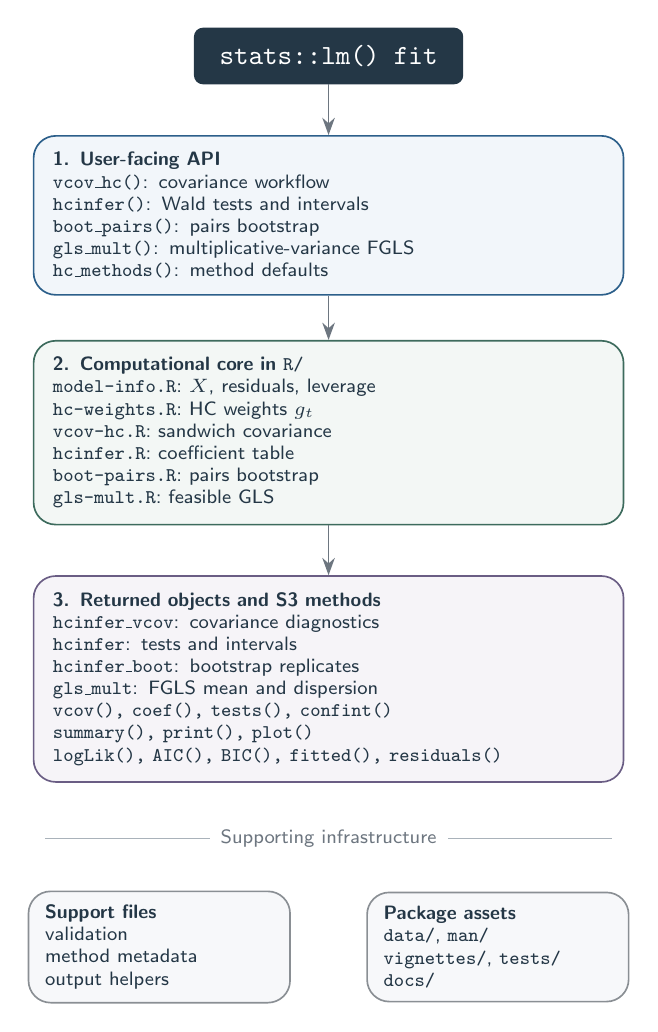
\begin{tikzpicture}[x=1cm,y=0.92cm]
  \node[hcentry, minimum width=34mm] (fit) at (0,8.2) {stats::lm() fit};

  \node[hccard, draw=hcapi, fill=hcapifill, text width=70mm, font=\scriptsize\sffamily, inner xsep=7pt, inner ysep=6pt] (api) at (0,6.0) {%%
    \textbf{1. User-facing API}\\
    {\bfseries\ttfamily vcov\_hc()}: covariance workflow\\
    {\bfseries\ttfamily hcinfer()}: Wald tests and intervals\\
    {\bfseries\ttfamily boot\_pairs()}: pairs bootstrap\\
    {\bfseries\ttfamily gls\_mult()}: multiplicative-variance FGLS\\
    {\bfseries\ttfamily hc\_methods()}: method defaults
  };

  \node[hccard, draw=hccorecol, fill=hccorefill, text width=70mm, font=\scriptsize\sffamily, inner xsep=7pt, inner ysep=6pt] (core) at (0,3.0) {%%
    \textbf{2. Computational core in \texttt{R/}}\\
    {\ttfamily model-info.R}: \(X\), residuals, leverage\\
    {\ttfamily hc-weights.R}: HC weights \(g_t\)\\
    {\ttfamily vcov-hc.R}: sandwich covariance\\
    {\ttfamily hcinfer.R}: coefficient table\\
    {\ttfamily boot-pairs.R}: pairs bootstrap\\
    {\ttfamily gls-mult.R}: feasible GLS
  };

  \node[hccard, draw=hcobject, fill=hcobjectfill, text width=70mm, font=\scriptsize\sffamily, inner xsep=7pt, inner ysep=6pt] (objects) at (0,-0.4) {%%
    \textbf{3. Returned objects and S3 methods}\\
    {\ttfamily hcinfer\_vcov}: covariance diagnostics\\
    {\ttfamily hcinfer}: tests and intervals\\
    {\ttfamily hcinfer\_boot}: bootstrap replicates\\
    {\ttfamily gls\_mult}: FGLS mean and dispersion\\
    {\bfseries\ttfamily vcov(), coef(), tests(), confint()}\\
    {\bfseries\ttfamily summary(), print(), plot()}\\
    {\bfseries\ttfamily logLik(), AIC(), BIC(), fitted(), residuals()}
  };

  \draw[hcsplit] (-3.6,-2.6) -- node[hclabel, fill=hcpage, inner xsep=4pt, inner ysep=1pt] {Supporting infrastructure} (3.6,-2.6);

  \node[hccard, draw=hcsupport, fill=hcsupportfill, text width=29mm, font=\scriptsize\sffamily, inner xsep=6pt, inner ysep=5pt] (support) at (-2.15,-4.1) {%%
    \textbf{Support files}\\
    validation\\
    method metadata\\
    output helpers
  };

  \node[hccard, draw=hcsupport, fill=hcsupportfill, text width=29mm, font=\scriptsize\sffamily, inner xsep=6pt, inner ysep=5pt] (assets) at (2.15,-4.1) {%%
    \textbf{Package assets}\\
    {\ttfamily data/}, {\ttfamily man/}\\
    {\ttfamily vignettes/}, {\ttfamily tests/}\\
    {\ttfamily docs/}
  };

  \draw[hcedge] (fit.south) -- (api.north);
  \draw[hcedge] (api.south) -- (core.north);
  \draw[hcedge] (core.south) -- (objects.north);
\end{tikzpicture}
\end{document}
